% vim: tw=0:wrap:linebreak
\documentclass[12pt]{article}

% \setcitestyle{numbers}
\usepackage[numbers]{natbib}
\usepackage[english]{babel}
\usepackage[utf8x]{inputenc}
\usepackage{datetime}
\usepackage{xspace}
\usepackage{graphicx}

\usepackage{titlesec}

\newcommand{\code}[1]{\texttt{#1}}
\newcommand{\DIASource}{\code{DIASource}\xspace}
\newcommand{\DIASources}{\code{DIASources}\xspace}
\newcommand{\DIAObject}{\code{DIAObject}\xspace}
\newcommand{\DIAObjects}{\code{DIAObjects}\xspace}
\newcommand{\SSObject}{\code{SSObject}\xspace}
\newcommand{\SSObjects}{\code{SSObjects}\xspace}

\title{Impact of a Hybrid Focal Plane on LSST Image Differencing}

\author{C. T. Slater, et al. }
%R. L. Jones, M. Juri\'c, E. Bellm


\begin{document}
\date{\today}
\maketitle


\section{Executive Summary}

If the LSST focal plane is comprised of sensors from multiple vendors, it is
likely that they will differ in quantum efficiency as a function of wavelength.
Based on preliminary throughput curves derived in early 2017 from engineering
models, the g-band exhibits the greatest difference between the two vendors,
particularly in the shape of the throughput curve. Thus the measured flux of an
object observed with one vendor's sensor will differ from that measured on the
other type of sensor, and the magnitude (and direction) of this effect will
depend on the spectral energy distribution of the object.

This problem is analogous to the issue of differential chromatic refraction (DCR),
where a similar sensitivity to the object's SED appears when an object is
observed at varying airmass. DCR is very challenging since it induces an
astrometric shift, rather than purely a photometric shift. DCR has been long
identified as a significant challenge for Data Management, and efforts at
developing algorithms to correct for this effect are underway. It is very likely
that an extension of the same algorithms designed for correcting DCR will also
be able to correct for the different sensor response curves, since they both
require estimating the coarse intra-band SED, then generating an appropriately
corrected template for image differencing. This would be the ideal solution for
handling the mixed-vendor focal plane.

We have also sought to characterize the degradation of image differencing
performance if a hybrid focal plane was used without such an algorithm in place
\footnote{We do not address the effects on the annual Data
Release Production, since the additional processing capability XXX}.
A significant concern is that images of an object from one sensor type may be
differenced against a template built from the other sensor type, leading to an
artificial difference in flux that would be reported as a \DIASource even if the
object is unvarying. If this occurs for a large number of objects it could
degrade the purity of the Level 1 alert stream, add excessive computational
cost, and potentially hamper the linking of moving object detections into
\SSObjects.

We have evaluated the magnitude of the flux difference in g-band for various
stellar SEDs. The shift can be ``calibrated out'' for stars of a median color,
since they will statistically set the zeropoint difference between the two
exposures. But stars significantly bluer or redder than this median color will
still exhibit flux shifts, and these are generally of order 5-10 mmag at most.
To determine how many stars fall into these red and blue wings, we use a
measured stellar color distribution from SDSS. Finally, for most faint stars
this shift will be lost in Poisson noise of the measurement, but bright stars
will be measured well enough they will be more likely to cross the $5\sigma$
threshold to be reported as a \DIASources. We therefore a modeled distribution
of observed stellar magnitudes plus a model of the photometric uncertainties for
stars with a given brightness and spurious flux shift (from the hybrid focal
plane) to estimate the total number of false positives per square degree.

The results from this exercise show that the worst-case false detection rates
from the hybrid focal plane are roughly 1-20 per square degree, depending on
whether the field is at low or high Galactic latitude. This is below the
irreducible level of detections from pure background noise of roughly 60/sq deg.
We therefore do not believe that the hybrid focal plane will present a problem
for image differencing.

However, the false positive rate rises very steeply with any such coherent
difference in flux between images. The filters are another potential source of
such differences, as localized variation in coatings could lead to a similar
dependence on object SED as described above. Based on the filter transmission
curve specifications, the magnitude of this effect is potentially much larger
than the differences between sensors. The filter bandpasses are permitted to
vary by up to 1.5\%, which in g-band would cause photometric differences as
large as 10-20 mmag. This could potentially create false positives at rates of
100s per square degree. Expected rates of astrophysical transients are of a
similar order of magnitude, which makes this a significant concern.



\section{Analysis}
\begin{figure}
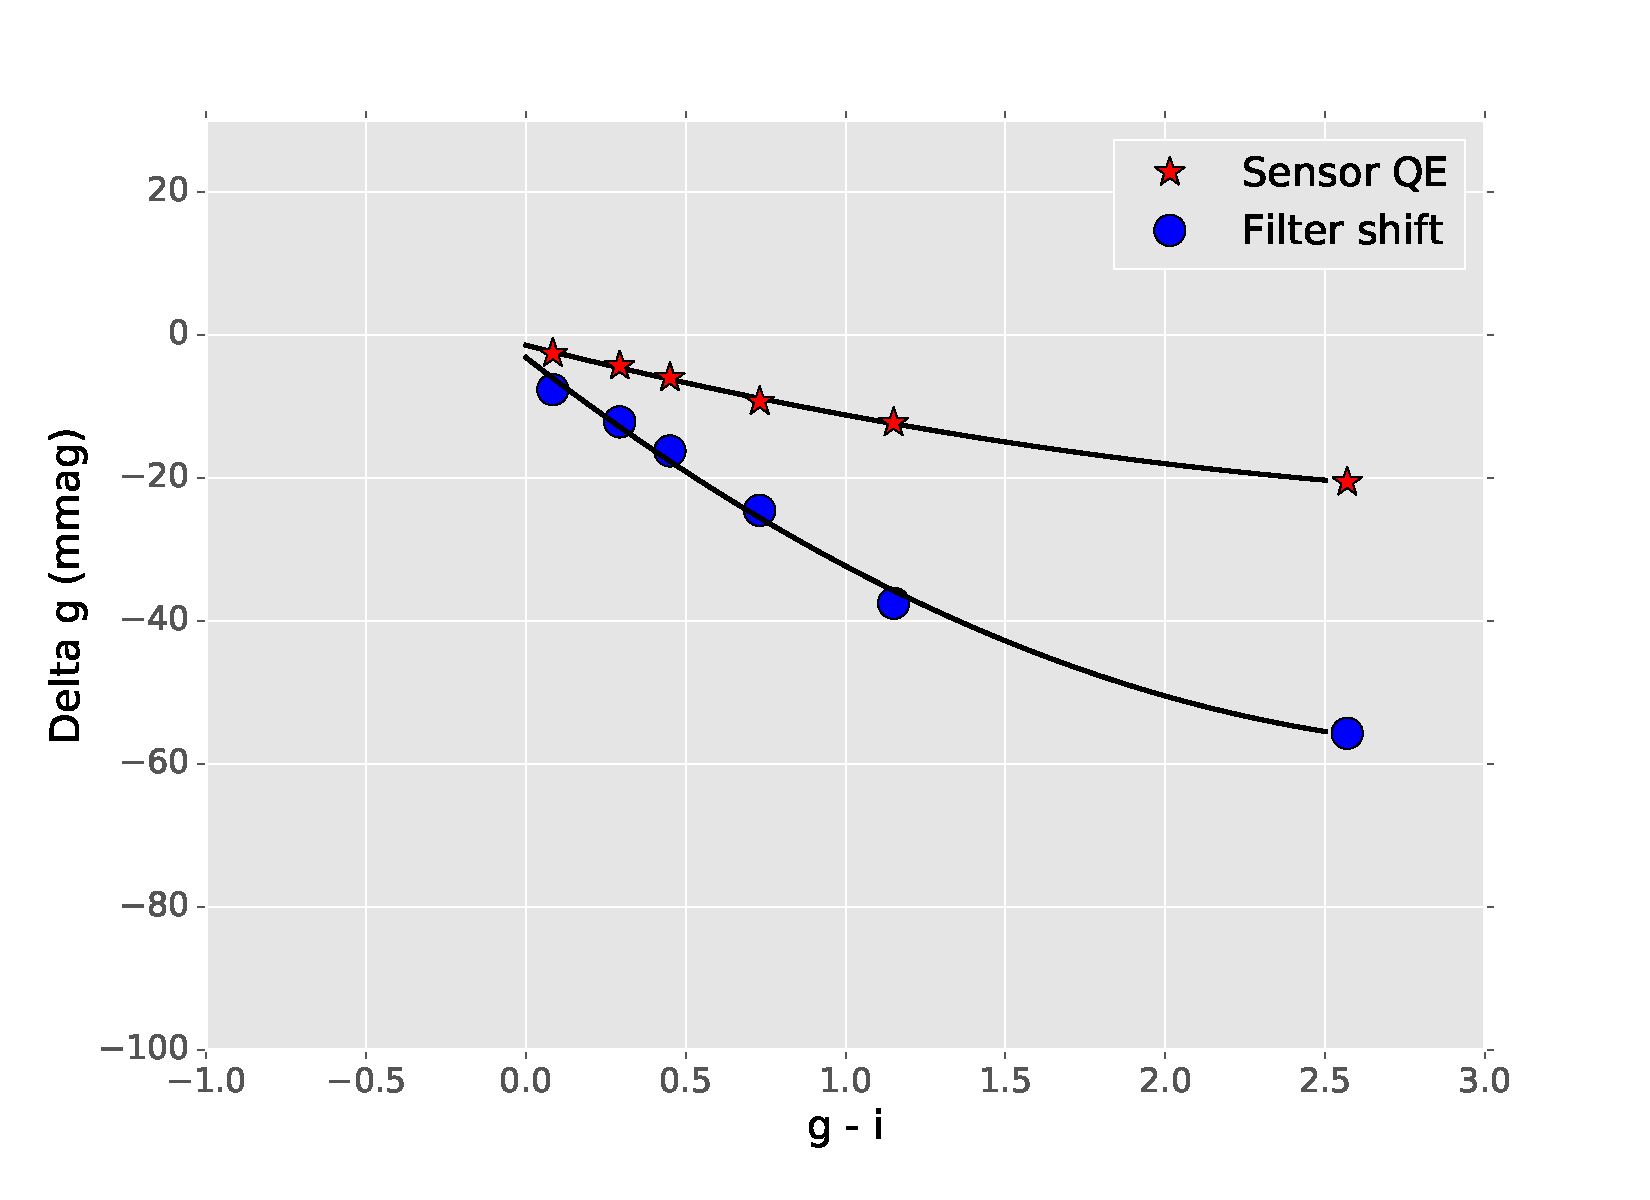
\includegraphics[width=0.9\textwidth]{figures/delta_g_vs_color.pdf}
\caption{Difference in g-band flux between measurements made on sensors from
different vendors (``Sensor QE'', red stars), and between two different
realizations of the g-band filter (``Filter shift''), where one filter
realization was the baseline specification and the other had both red and blue
cutoffs shifted by 1\% in wavelength (less than the 1.5\% specification). The
sensor QE curves used measured throughputs from prototype sensors as early
Spring 2017.
\label{fig:delta_g_vs_color}}
\end{figure}

\begin{figure}
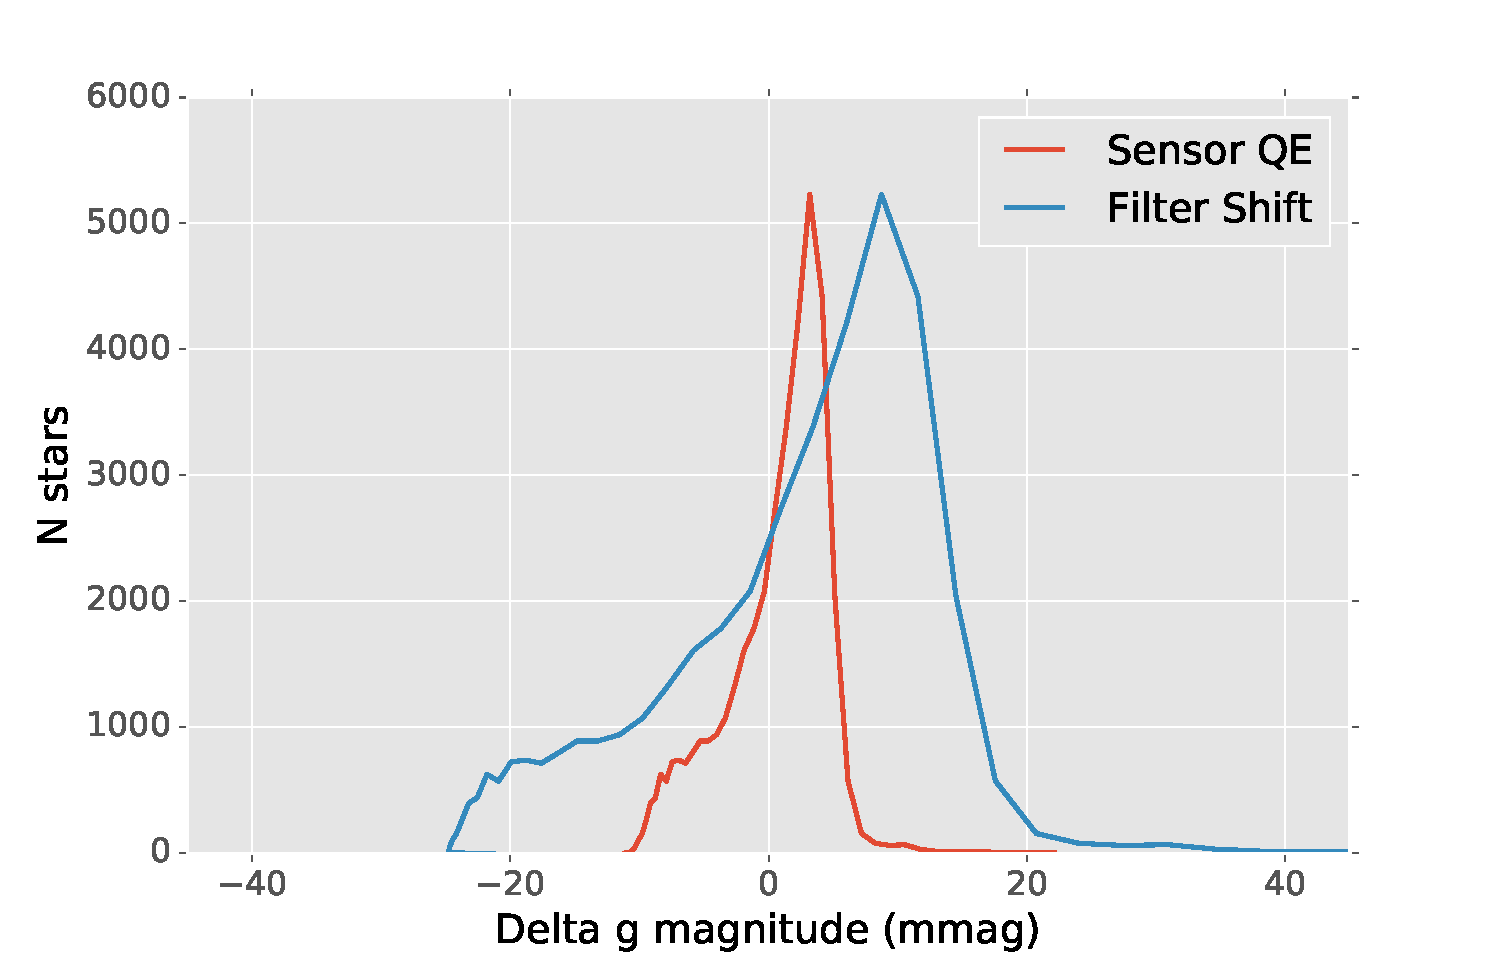
\includegraphics[width=0.9\textwidth]{figures/delta_g_histogram.pdf}
\caption{Distribution of g-band magnitude shifts that would be when stars with a
realistic $g-i$ color distribution were observed in the sensor and filter
scenarios described in Figure~\ref{fig:delta_g_vs_color}. The mean g-band
difference is removed when the two (hypothetical) images are matched in flux,
but very red or very blue stars will exhibit flux differences of up to $\sim 20$
mmag.
\label{fig:delta_g_histogram}}
\end{figure}

\begin{figure}
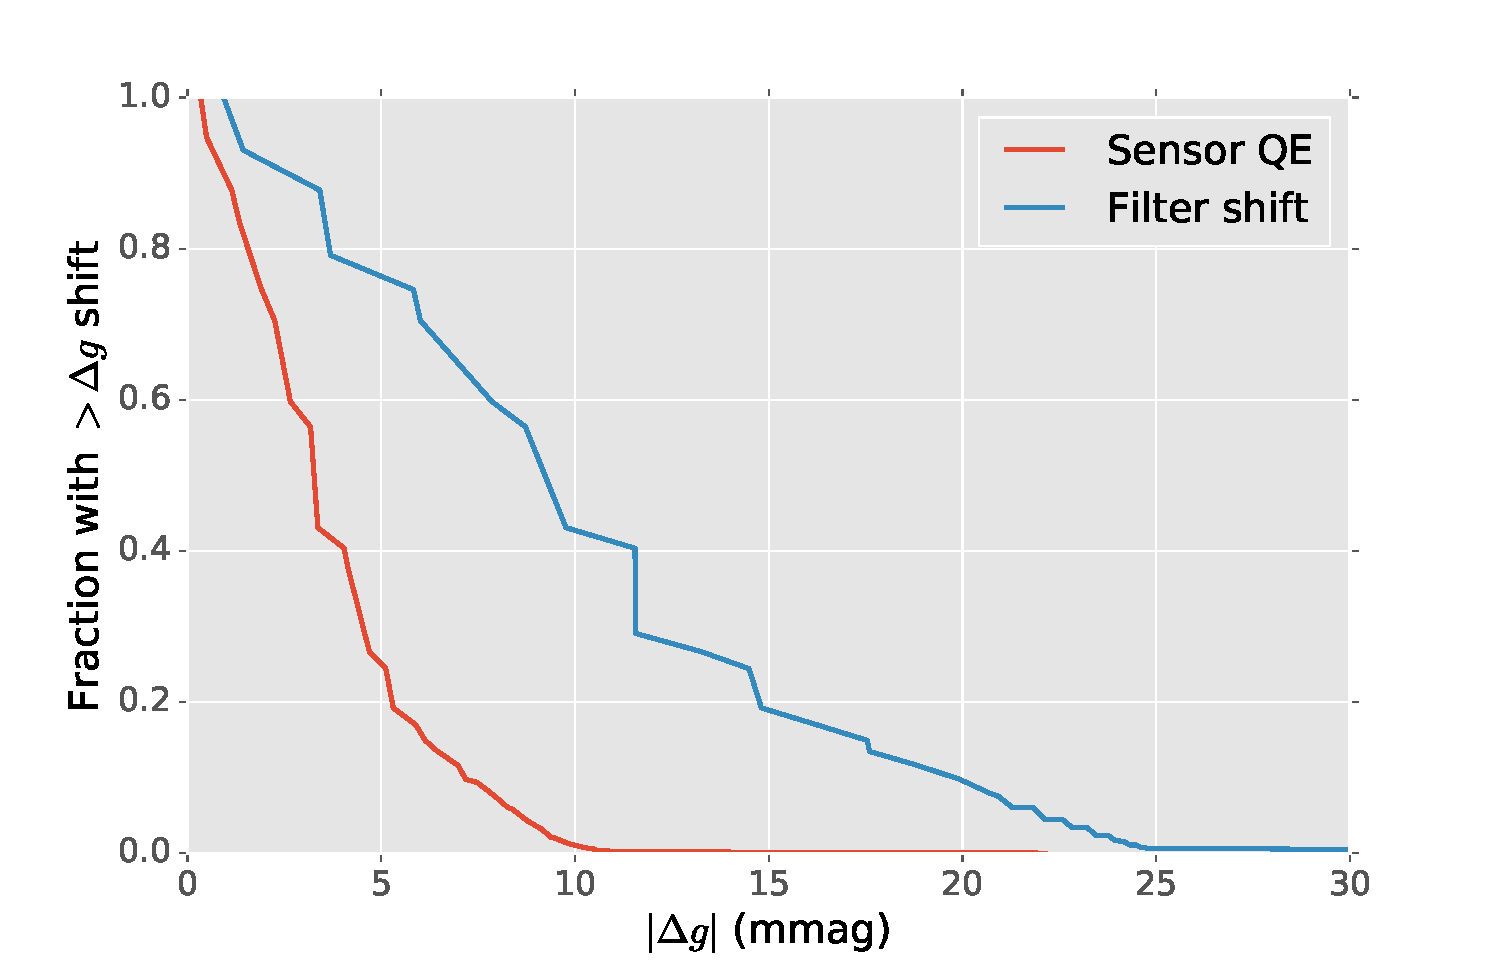
\includegraphics[width=0.9\textwidth]{figures/delta_g_cumulative.pdf}
\caption{Cumulative distribution of Figure~\ref{fig:delta_g_histogram}. Roughly
10-15\% of (unvarying) stars will exhibit $>7$ mmag g-band differences when
images from the two sensor types are differenced, while 20\% of stars will show
differences of $15$ mmag or greater if imaged by different filter bandpasses.
\label{fig:delta_g_cumulative}}
\end{figure}


\begin{figure}
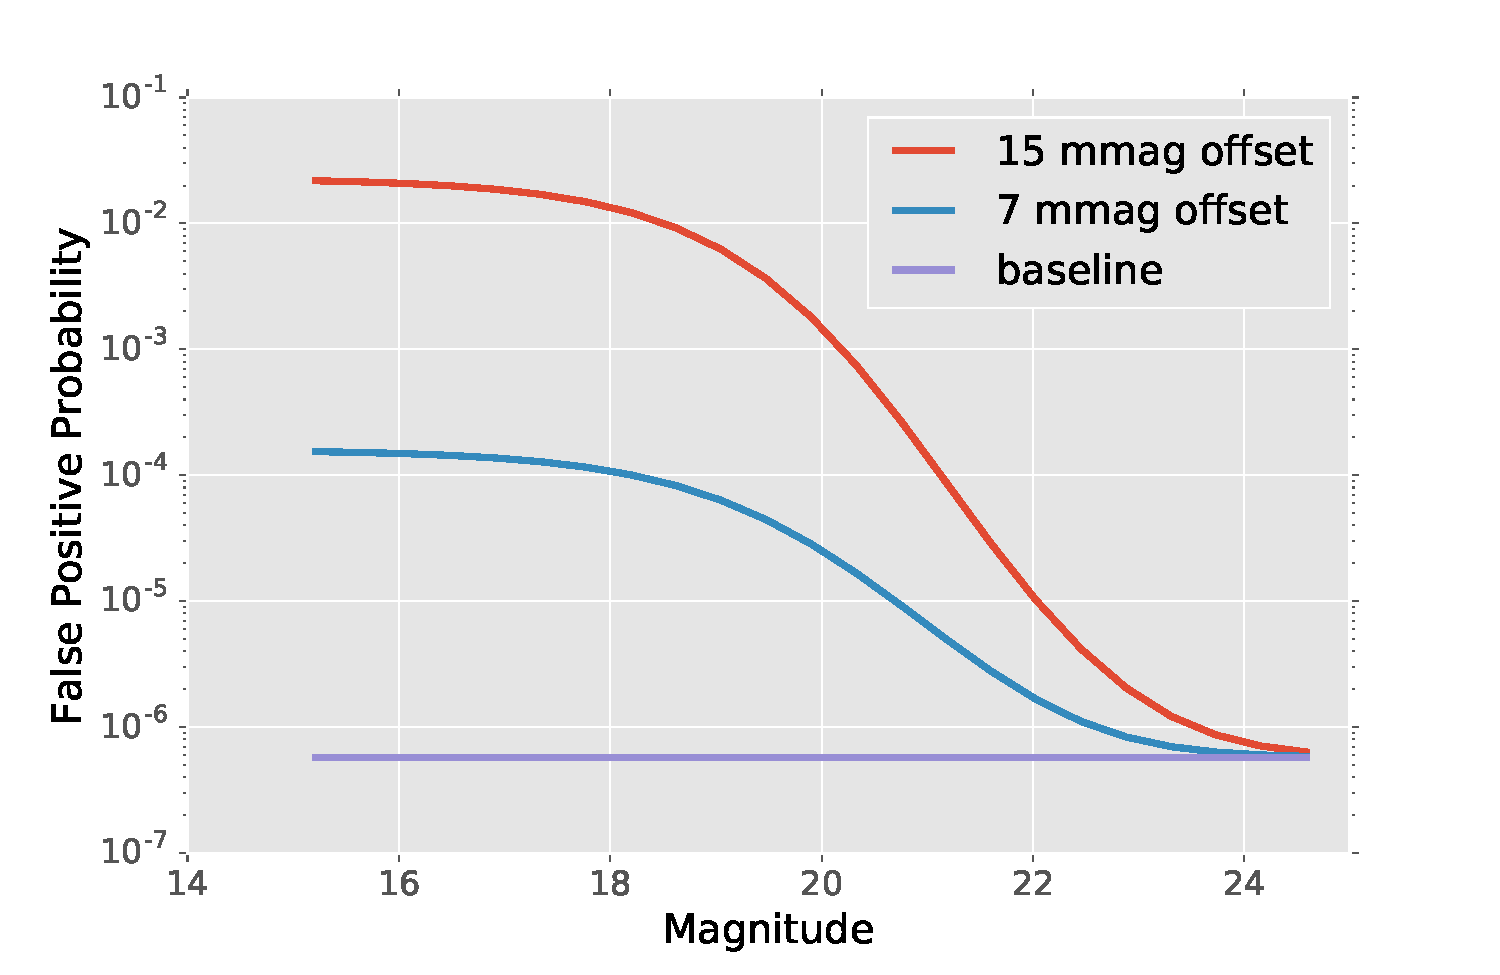
\includegraphics[width=0.9\textwidth]{figures/false_positive_prob.pdf}
\caption{Probability that a star at a given magnitude (unvarying) will be
measured as exceeding the $5\sigma$ threshold for \DIASources, if there is a
coherent flux difference between the two images that are differenced. These
false positives are rejected at better than 1 in $10^6$ when the two images have
the same bandpass and sensor QE curves, but when there are variations in the
transmission curve, bright stars will be significantly more likely to exceed the
$5\sigma$ threshold.
\label{fig:false_positive_prob}}
\end{figure}

\begin{figure}
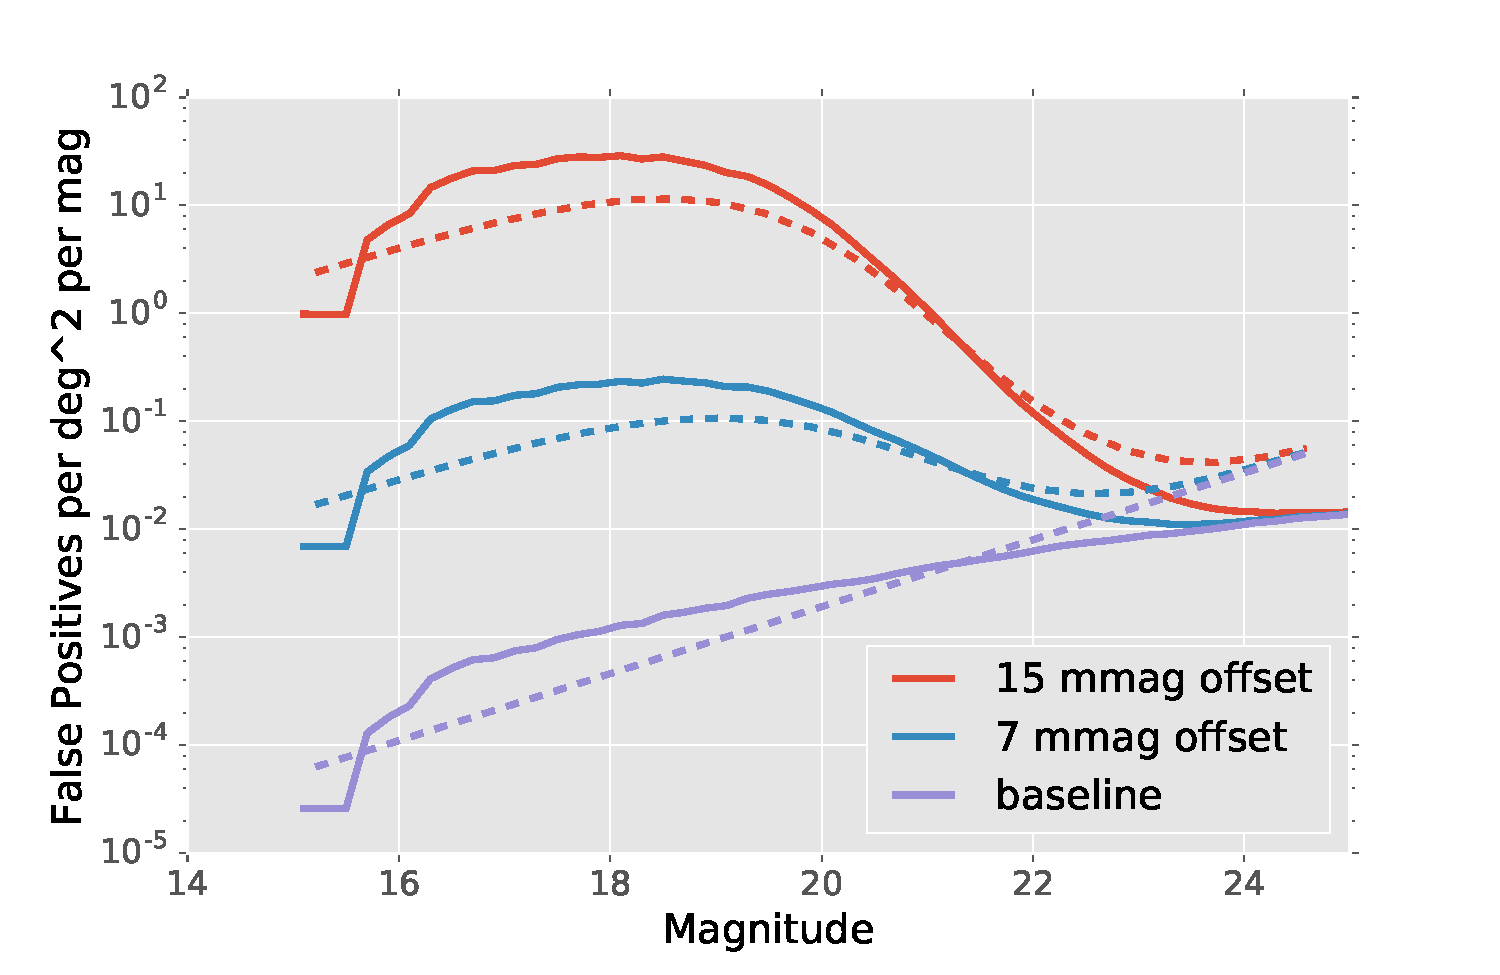
\includegraphics[width=0.9\textwidth]{figures/false_positive_differential.pdf}
\caption{This figure combines the false positive probabilities from
Figure~\ref{fig:false_positive_prob} with the number density of objects at a
given magnitude to show the total number of objects per square degree, per magnitude.
Solid lines show star counts (computed at $l=180^\circ$, $b=-45^\circ$), while
dashed lines show galaxies.
\label{fig:false_positive_differential}}
\end{figure}

\begin{figure}
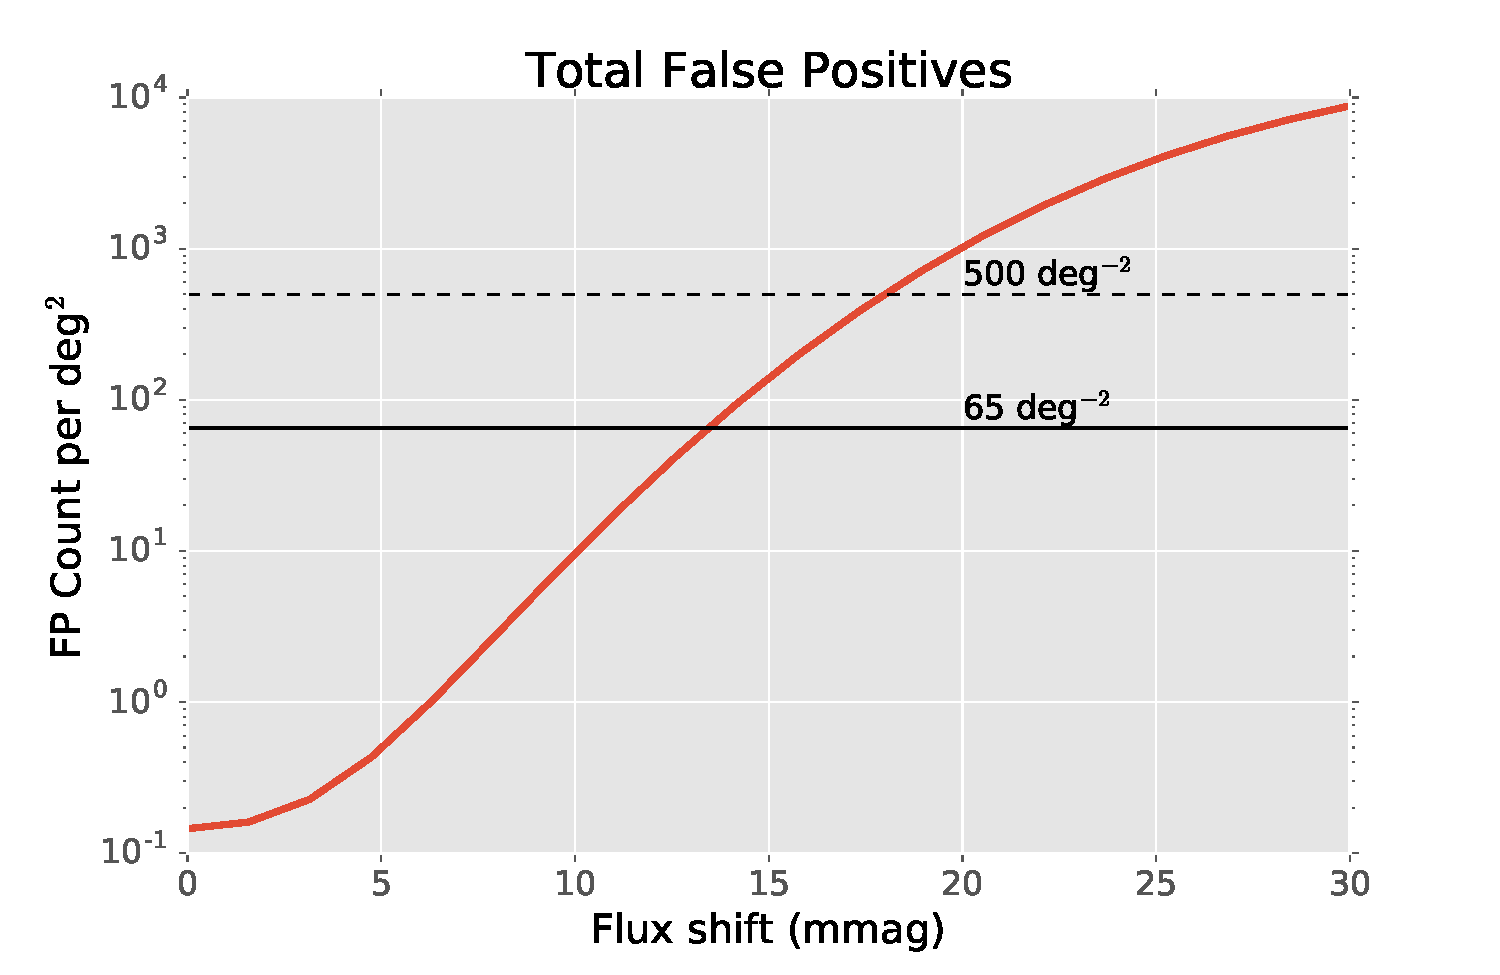
\includegraphics[width=0.9\textwidth]{figures/fp_vs_flux_shift.pdf}
\caption{Cumulative counts of false positives (stars exceeding $5\sigma$) as a
function of coherent flux difference between observations. While shifts of up to
12 mmag would not produce more false positives than the irreducible background
level of $\sim 65$ per square degree, greater shifts will would rapidly produce
significant numbers of false detections. \label{fig:fp_vs_flux_shift}}
\end{figure}

\end{document}
